\usepackage{beamerthemesplit}
\usepackage{graphicx}
\usepackage{pstricks}
\usepackage{tabularx, multirow, booktabs}
\usepackage{changepage}
\usepackage{color}
\usepackage{templates/pdfpcnotes}

\setbeameroption{hide notes}

\setbeamersize{text margin left=0pt,text margin right=0pt}

\definecolor{BigSQLGrey}{RGB}{116,116,116}

\setbeamercolor*{structure}{fg=BigSQLGrey}
\setbeamercolor{alerted text}{use=structure,fg=structure.fg}
\setbeamercolor*{palette primary}{use=structure,fg=structure.fg}
\setbeamercolor*{palette secondary}{use=structure,fg=structure.fg!95!black}
\setbeamercolor*{palette tertiary}{use=structure,fg=structure.fg!90!black}
\setbeamercolor*{palette quaternary}{use=structure,fg=structure.fg!95!black,bg=black!80}

\setbeamertemplate{background canvas}
{
  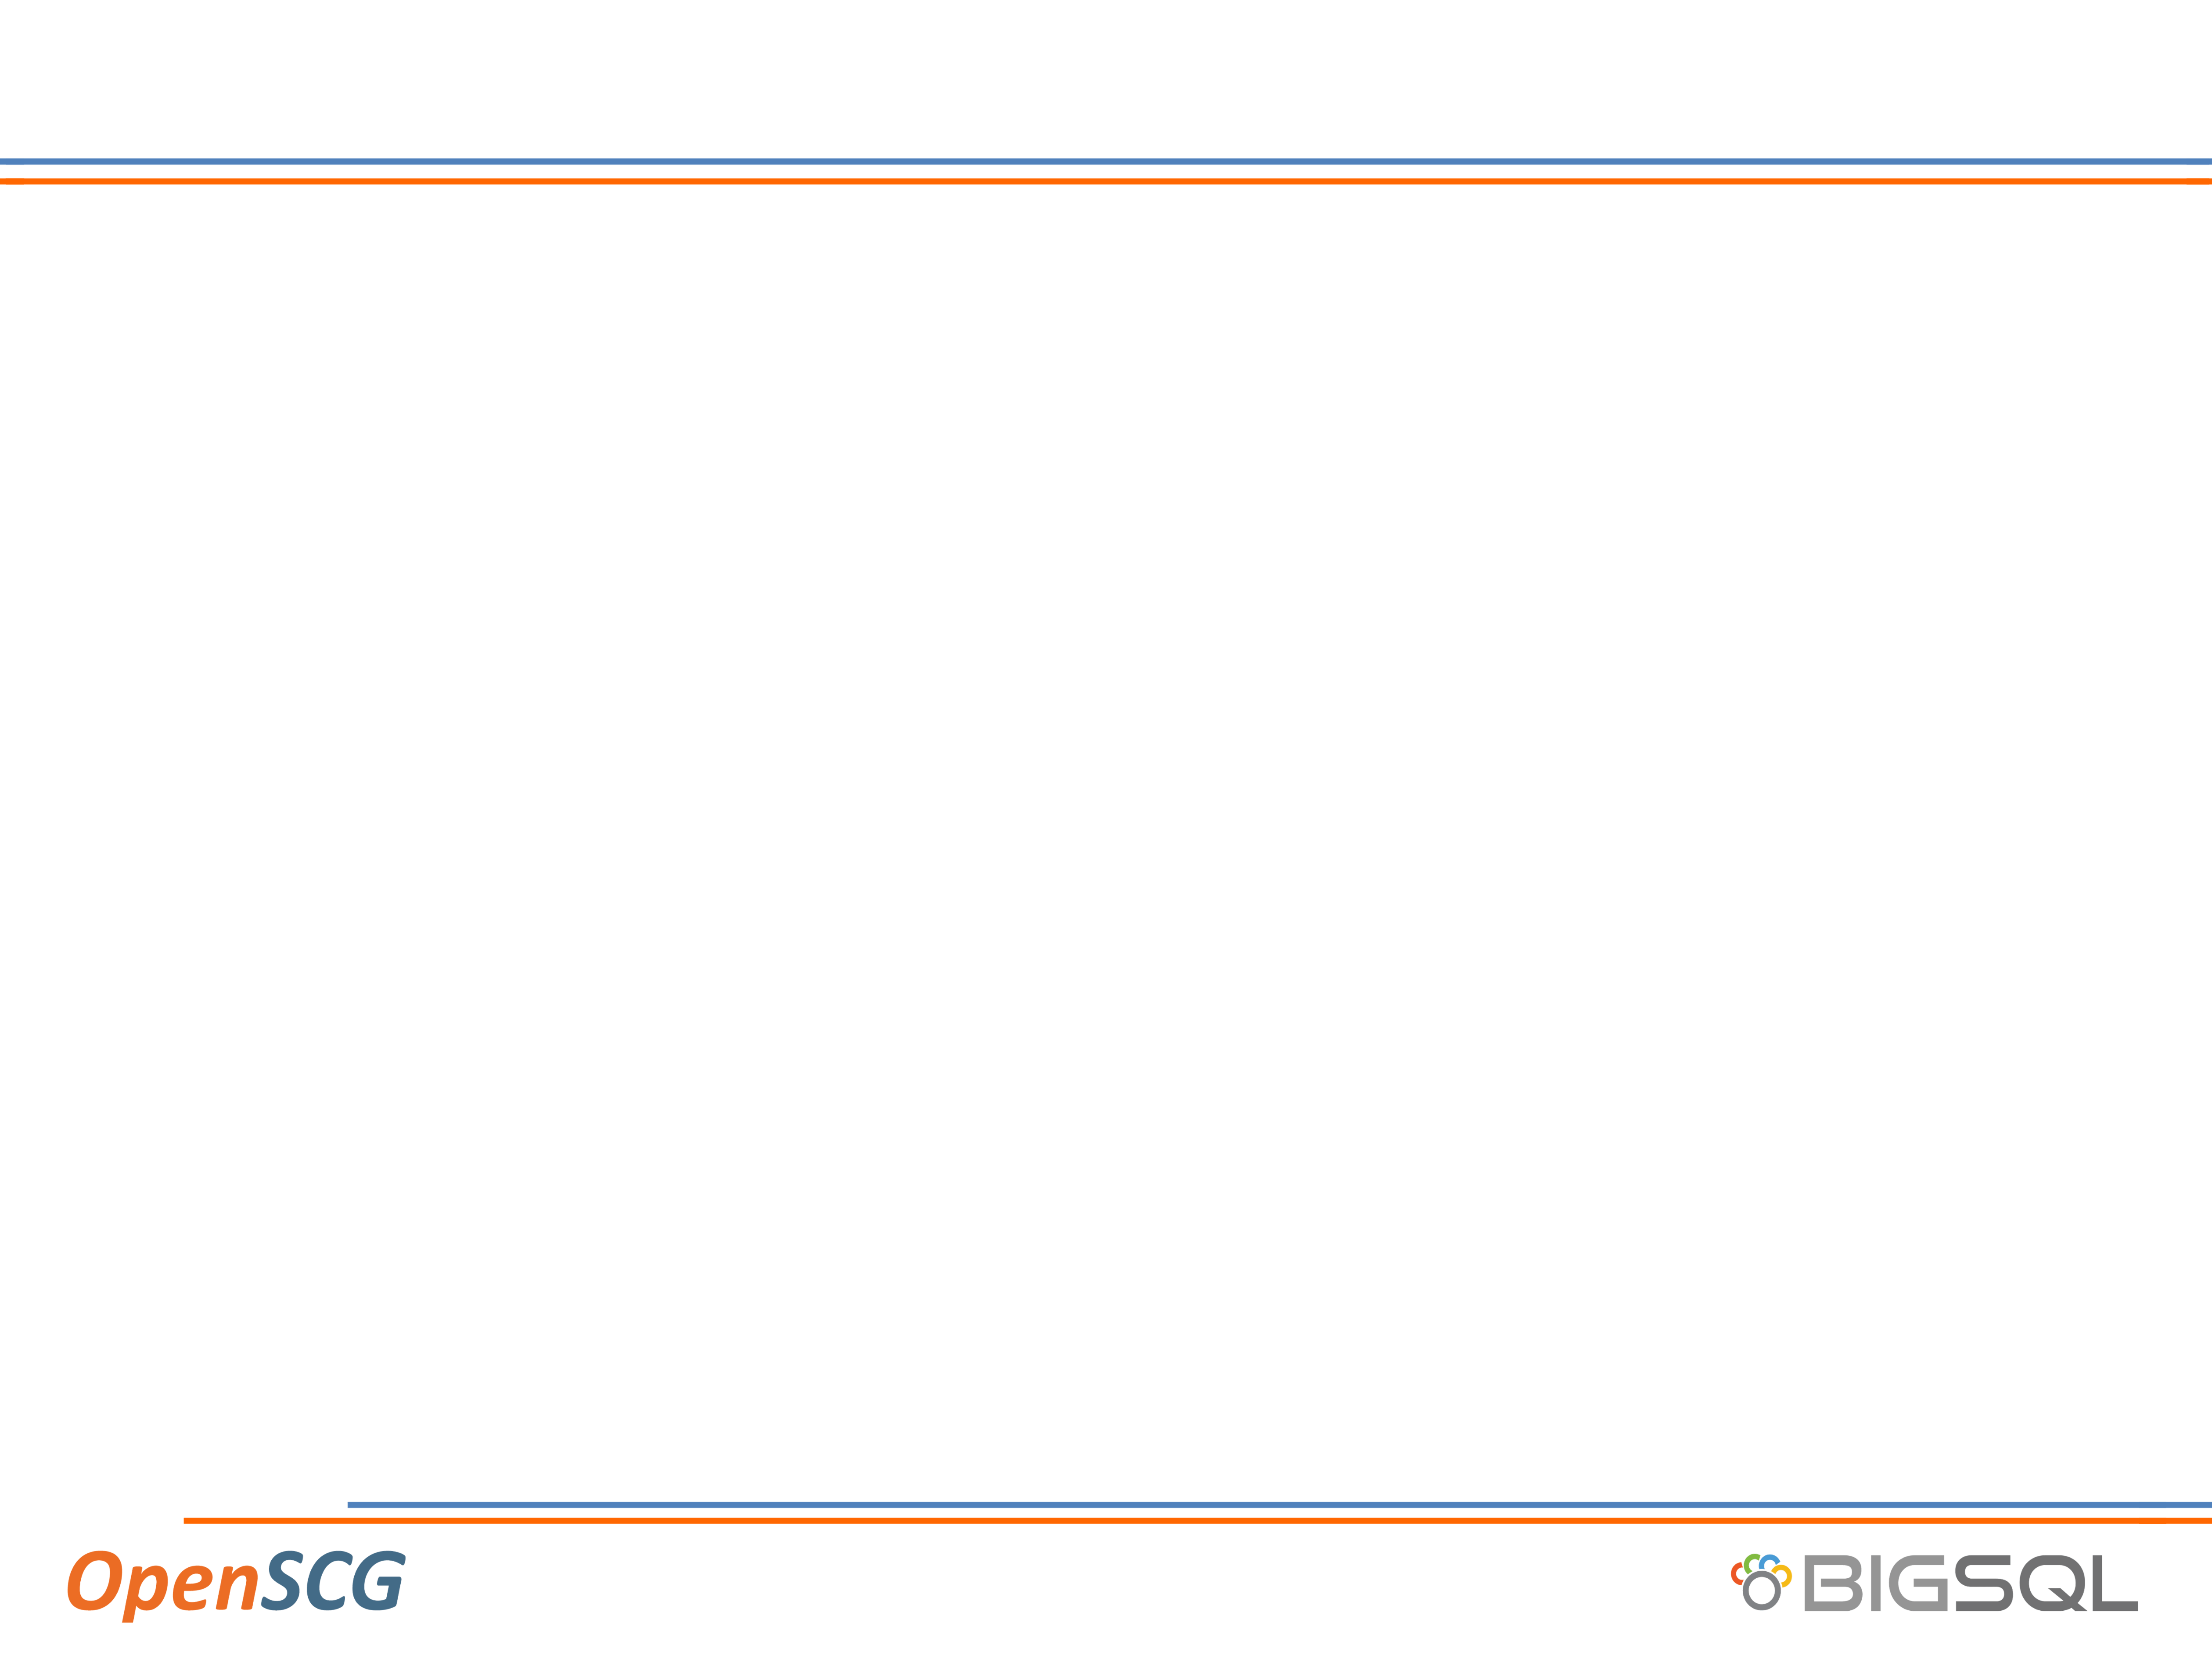
\includegraphics[width=\paperwidth,height=\paperheight]{./images/background.png}
}

\setbeamercolor*{framesubtitle}{fg=white}

\setbeamertemplate{itemize items}[circle]

\usefonttheme{professionalfonts}
\usepackage{setspace}
\linespread{1.10}
\setmainfont[Ligatures=TeX,Scale=1.20]{Arial}
\setsansfont[Ligatures=TeX,Scale=1.20]{Arial}
\setmonofont[Ligatures=TeX,Scale=0.80]{Courier}
\setbeamerfont{quote}{shape=\upshape}

\setbeamertemplate{footline}{}

% eliminate silly beamer navigation line at bottom of slides
\setbeamertemplate{navigation symbols}{}

\date{}

% ensure text jusfication
\usepackage{ragged2e}
\justifying

% pandoc makes 2nd-lever headers into blocks, and this ensures justification
% in blocks too
\addtobeamertemplate{block begin}{}
{
  \justifying
}


\urlstyle{same}
\usepackage[overlay,absolute]{textpos}

%\TPGrid[0 mm,0 mm]{9}{8}
% beamer's left and right margin is 10 mm. The top/bottom margin is ??
% or without a header ??
% the slide dimensions are 128 mm x 96 mm
% so the resulting \TPHorizModule = 12 mm and \TPVertModule = 10 mm



